\documentclass{standalone}
\usepackage{tikz}
\usepackage{ctex,siunitx}
\setCJKmainfont{Noto Serif CJK SC}
\usepackage{tkz-euclide}
\usepackage{amsmath}
\usepackage{wasysym}
\usetikzlibrary{patterns, calc}
\usetikzlibrary {decorations.pathmorphing, decorations.pathreplacing, decorations.shapes,}
\begin{document}
\small
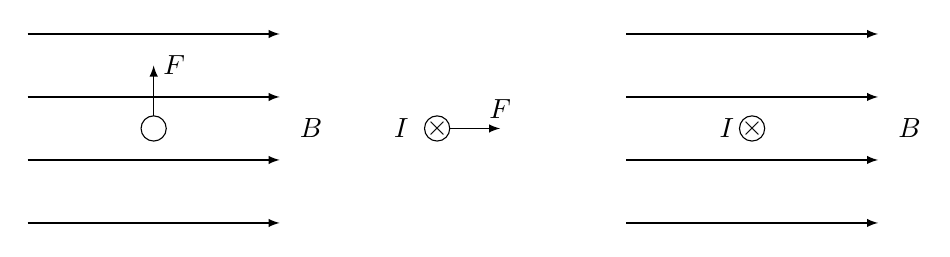
\begin{tikzpicture}[>=latex,scale=0.8]
  \useasboundingbox(0,0.9)rectangle(14.2,4.1);
  \foreach \x in {1,2,3,4}
  {
    \draw[->] (0,\x)--(4,\x);
    \draw[->] (9.5,\x)--(13.5,\x);
  }
  \draw[->](2,2.7)--(2,3.5)node[right]{$F$};
  \node at (4.5,2.5){$B$};
  \draw (2,2.5) circle (0.2);
  \draw[->](6.7,2.5)node[left=4mm]{$I$}--(7.5,2.5)node[above]{$F$};
  \draw (6.5,2.5) circle (0.2);
  \node at (6.5,2.5){$\times$};
  \draw (11.5,2.5) circle (0.2);
  \node at (11.5,2.5){$\times$};
  \node at (14,2.5){$B$};\node at (11.1,2.5){$I$};
\end{tikzpicture}
\end{document}